\chapter{Why DNA Suits Information Storage}

\begin{kaichang}
Your kitchen can host an experiment that sounds like science fiction. Mash a ripe strawberry in a food-storage bag, add a little salt water and a few drops of dishwashing liquid, swirl gently, and filter the juice through gauze. Slowly pour chilled alcohol over the filtrate and wait a few minutes. A white, cottony clump emerges at the interface, like a little bundle of thread. Touch it with a chopstick tip, and you can wind it up, gathering more and more.

First, guess: what is this white thread? Protein? Sugar? Fruit fibers?

None of those. It is strawberry DNA, hereditary molecules released from billions of cells. With a chopstick, you have fished life's ``instruction manual'' out of the water. This chapter asks what that molecule looks like, and why its particular appearance suits the job of ``storing information.''
\end{kaichang}

\section{Fishing White Threads from a Strawberry}

First describe only what your eyes and hands detect. The white clump is sticky and stringy, winding around a chopstick like transparent fishing line. It dissolves in water but not cold alcohol, so it ``appears'' where alcohol meets juice: first a thin haze, then gathering strands. The filtrate is pink, but the strands are white, showing they are neither pigment nor pulp. Riper, more thoroughly mashed strawberries yield more strands. There is a hidden reason to choose strawberries: cultivated strawberries are octoploid, with eight chromosome sets per cell (Chapter 64's hereditary ``shipping containers''). Their DNA content is much higher than that of ordinary fruit, making them particularly suitable.

\begin{shiyan}
\textbf{Materials}: two or three ripe strawberries, salt, water, dishwashing liquid, gauze or a coffee filter, a transparent drinking glass, medical alcohol (chilled beforehand in the freezer, but not frozen solid), and a chopstick.

\textbf{Steps}: (1) Remove the strawberry tops, bag the fruit, and mash it. (2) Dissolve a small spoonful of salt in half a cup of warm water, add a few drops of detergent, pour into the bag, and swirl gently for two minutes without shaking up foam. (3) Filter through gauze into the glass. (4) Slowly pour an equal volume of cold alcohol down the glass wall and wait 5 minutes. (5) Gently stir at the interface with the chopstick tip and wind up the strands.

\textbf{Observations}: how quickly strands appear, whether they stretch into threads, and their different solubility in alcohol and water. Why add salt? Why cold alcohol?

\textbf{Safety}: Alcohol is flammable: keep flames away throughout. Do not eat experimental materials. Keep detergent out of your eyes. This experiment can be done at home, but wash your hands afterward.
\end{shiyan}

\textbf{Translator safety note:} Do not follow the source's household-freezer instruction: ordinary refrigerators and freezers can ignite flammable vapors and are not rated for flammable-chemical storage. See \href{https://ehs.stanford.edu/wp-content/uploads/Lab-Compliance-Cheat-Sheet.pdf}{Stanford laboratory safety guidance}. Have a qualified teacher select a safe preparation and chilling procedure, with adult handling, eye protection, no heat or ignition sources, and no tasting; see \href{https://www.acs.org/education/celebrating-chemistry-editions/2024-ccew/science-safety-tips.html}{ACS activity precautions}. The white precipitate is a crude mixture, not purified DNA identified by appearance alone.

What you cannot see is that a ``thread'' is not one molecule, but hundreds of millions of extremely long molecules tangled together. A single DNA molecule is only about 2 nanometers thick, hundreds of times smaller than visible light's wavelength; no light microscope can resolve its details. The method also works with bananas, onions, and peas: materials with plenty of cells and DNA yield white threads, though strawberries are particularly generous. To see the molecule's appearance clearly, zoom down to atoms.

\section{Zooming In: One Nucleotide}

DNA is a polymer, a large molecule made of many repeating units (like Chapter 43's plastics and Chapter 46's starch). Its repeating unit is the \textbf{nucleotide}, a three-in-one building block:

\begin{itemize}[itemsep=2pt]
\item A \textbf{phosphate}: the oxygen-containing phosphorus acid group from Chapter 14, negatively charged in water.
\item A \textbf{deoxyribose}: a small ring of five carbon atoms, belonging to the sugars (Chapter 46), with one fewer oxygen than ribose---hence ``deoxy.''
\item A \textbf{base}: a flat, nitrogen-containing ring molecule (Chapter 14's nitrogen meets Chapter 41's aromatic rings), the part that actually bears the ``letter.''
\end{itemize}

You have already ``eaten'' and ``used'' nucleotides. ATP, Chapter 50's energy currency, is an adenine nucleotide carrying three phosphates. The flavor-enhancing nucleotides in shiitake mushrooms and chicken broth are relatives. Nucleotides are not laboratory rarities but among life's most universal components. ``Nucleic acid'' is a historical name: first isolated from nuclei, the material is acidic thanks to backbone phosphates.

There are only four bases: adenine (A), guanine (G), cytosine (C), and thymine (T). A and G have two rings, are larger, and are called purines. C and T have one ring, are smaller, and are called pyrimidines. These four letters form DNA's entire alphabet.

How do nucleotides form a chain? Phosphates act as connectors, joining one deoxyribose to the next. The chain's ``keel'' is therefore an alternating sugar--phosphate backbone, with bases projecting like flags from each sugar. Remember two properties: negatively charged phosphates make the backbone hydrophilic and attracted to positive ions, while the projecting flat-ring bases are comparatively ``water-shy'' (recall Chapter 47's hydrophobic lipids). These properties will determine how two chains embrace.

\section{Rule One: Direction and Pairing Matter}

First, direction. Deoxyribose's five carbon atoms are conventionally numbered $1'$ through $5'$ (``one prime'' to ``five prime''). Phosphate always joins one sugar's $3'$ carbon to the next sugar's $5'$ carbon, link after link. The whole chain gains a head and tail: a free $5'$ phosphate at the $5'$ end, and a free $3'$ group at the $3'$ end. Like train carriages facing front and back and a train with a head and tail, DNA has direction. Its copying and reading machinery must recognize that direction before starting.

Next, pairing. In two side-by-side strands, bases face each other under strict rules: A pairs only with T through two hydrogen bonds; G pairs only with C through three. (Hydrogen bonds are the weak intermolecular interactions in Chapters 22 and 23.) Why these partners? Their hydrogen-bond ``donors'' and ``acceptors'' complement each other like plugs and sockets: A's projecting hydrogen faces T's lone electron pair; swap partners and the positions do not match. Geometry matters too: pairing a large purine with a small pyrimidine gives almost equal widths, keeping the double strand uniformly about 2 nanometers thick rather than uneven.

Finally, the strands' relative direction: they are \textbf{antiparallel}. One runs $5'$ to $3'$, the other $3'$ to $5'$, like escalators traveling in opposite directions. This apparently minor detail becomes the copying machinery's ``Achilles' heel'' in Chapter 67. Remember it.

Revisit Chargaff's rule from Chapter 65: in double-stranded DNA from any source, A equals T and G equals C. Once a puzzling statistical observation, it becomes inevitable in the pairing model: every A holds a T across the strand. A good theory does more than explain new phenomena; it turns old mysteries into ``of course.''

The strands do not merely lie side by side. Once paired, the double strand naturally twists into a helix, roughly 10 base pairs per turn: the \textbf{double helix} revealed by Chapter 65's X-ray diffraction images. That chapter asked how scientists knew; this one asks why the structure suits information storage.

\section{Rule Two: Weakness Is the Clever Part}

The first instinct is that stored information should be as secure as possible, with strands ``glued'' immovably together. The opposite is true. DNA's ingenuity combines ``weak'' with ``many.''

\begin{qiaoliang}
Compare energy scales. A hydrogen bond's binding energy is only about \ud{10\sim 20}{kJ\,mol^{-1}}, versus roughly \ud{350}{kJ\,mol^{-1}} for a covalent bond. Average molecular thermal energy at body temperature is on the order of \ud{2.5}{kJ\,mol^{-1}}. A handful of hydrogen bonds can therefore be shaken apart at any time. Indeed, DNA constantly ``breathes'' locally at body temperature: short paired segments open and close. But a 1000-base-pair segment has two or three thousand hydrogen bonds, and shaking them all apart simultaneously is negligibly unlikely. Like a zipper, one tooth opens with a nudge while the whole zipper is secure; deliberately opening it tooth by tooth from one end is easy. Another quieter contribution comes from base stacking: flat bases pile like coins. Van der Waals forces between rings, plus stabilization from water-shy bases hiding inside the helix away from water (the hydrophobic effect of Chapters 23 and 47), are the main source of overall helical stability. Hydrogen bonds ``recognize partners,'' ensuring A finds T; stacking ``holds the group together,'' keeping the structure intact. Specificity and stability divide the work.
\end{qiaoliang}

We can now answer half our title. At least three structural features suit DNA to information storage:

\begin{itemize}[itemsep=2pt]
\item \textbf{Few letters, unrestricted sequences}. The backbone is uniform, but the four bases may occur in any order, allowing any ``text.''
\item \textbf{Each strand is a complete backup}. Pairing rules uniquely determine one strand from the other's sequence. Information has two copies, and the copies can separate.
\item \textbf{Many weak bonds permit reading and writing}. For copying or repair, molecular machines open the double strand locally like a zipper, assemble a complementary strand using one as a template, then close it again. ``Many weak interactions'' simultaneously satisfy apparently conflicting demands: secure storage and ready access.
\end{itemize}

The second feature also addresses ``what if something breaks?'' If a base on one strand is damaged, the cell can consult the intact strand as an answer key for repair. Damage and repair are among next chapter's topics. For now, remember the structural setup: complementary strands come with a built-in correction copy.

\section{Writing the Helix as a Line of Letters}

After all this preparation, symbols may finally appear. Because the backbone is always the same and pairing fixed, biologists simply write one strand's base sequence and direction, for example:

\[5'\text{-ATGCGTAC-}3'\]

Its partner follows directly from the rules, with the opposite direction:

\[3'\text{-TACGCATG-}5'\]

Here is the double helix as a ``ladder'' (a human representation: real bases are not letters, and molecules have no colors):

\begin{center}
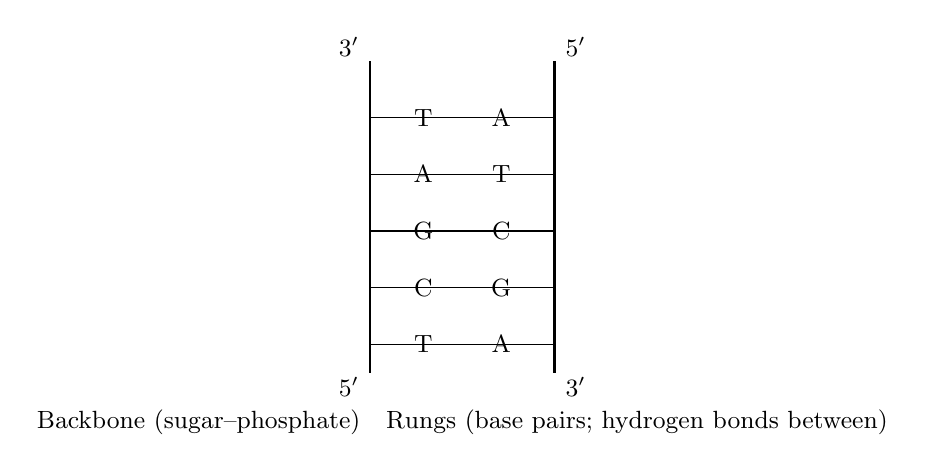
\begin{tikzpicture}[scale=0.9]
\draw[thick] (0,0) -- (0,4.4);
\draw[thick] (2.6,0) -- (2.6,4.4);
\foreach \y/\a/\b in {0.4/T/A, 1.2/C/G, 2.0/G/C, 2.8/A/T, 3.6/T/A}{
  \draw (0,\y) -- (2.6,\y);
  \node at (0.75,\y) {\small \a};
  \node at (1.85,\y) {\small \b};
}
\node at (-0.3,4.6) {\small $3'$};
\node at (-0.3,-0.2) {\small $5'$};
\node at (2.9,4.6) {\small $5'$};
\node at (2.9,-0.2) {\small $3'$};
\node at (1.3,-0.7) {\small Backbone (sugar--phosphate)\quad Rungs (base pairs; hydrogen bonds between)};
\end{tikzpicture}
\end{center}

Notice the opposite direction labels on the vertical lines: that detail encodes antiparallel orientation. The real molecule twists into a helix, but information lies in the rung sequence. The helix is simply the ladder's most compact, stable storage form.

How much information fits in a letter sequence? Four choices at each of $n$ positions give $4^n$ sequences. Ten positions already exceed a million ($4^{10}\approx 1.05\times 10^{6}$). One human genome set has about $3\times 10^{9}$ base pairs, allowing four to the three-billionth power possible sequences. Writing that number would require more paper than the observable universe. A more tangible calculation: printing three billion letters at 1000 per page takes three million pages, or 6000 books of 500 pages. Almost every cell carries such a library---twice, thanks to Chapter 64's diploidy.

The letters also occupy physical space. Adjacent base pairs lie 0.34 nanometers apart. One genome set stretches about $3\times 10^{9}\times 0.34$ nanometers, roughly one meter; two sets, two meters. A nucleus just six micrometers across must contain those two meters. We will settle that account at the chapter's end.

``Sequence is information'' has long since left the laboratory for familiar news technologies. Paternity testing compares several short variable sequences: every segment in a child must trace to one parent (Chapter 63's probability becomes courtroom evidence). Forensic DNA fingerprints work similarly, matching molecules in a hair or saliva trace with database sequences. Nucleic acid testing takes another approach: a synthetic short DNA strand acts as a ``probe,'' exploiting ``A recognizes only T, G only C.'' A complementary viral sequence in the sample binds the probe and produces a signal. None of these techniques needs a clear molecular picture; all depend only on sequence carrying information and pairing being specific.

\section{Heat It, and the Evidence Appears}

\begin{zhengju}
The double-helix drawing is beautiful, but how can we test whether bases pair through weak bonds and separate reversibly? A much cheaper experiment answers: slowly heat an aqueous DNA solution while measuring ultraviolet absorption.

Bases absorb ultraviolet near 260 nanometers, with a subtle twist: neatly stacked inside a helix, they absorb less. Separate the strands and expose the bases, and absorption rises markedly, by up to about forty percent. In the late 1950s, researchers including Marmur and Doty used this effect to plot DNA ``melting curves.'' As temperature rises, absorption initially barely changes, then climbs sharply near a certain temperature. Like ice melting, the double strands open into single strands within this interval. The temperature is called the melting temperature, $T_m$.

The first key finding: DNA from different sources has different $T_m$, and higher G and C content makes it more ``heat-resistant,'' in an almost linear relationship. Why is this evidence? Some unspecified glue would have no reason to track G and C proportions. In the pairing model, however, G--C pairs have three hydrogen bonds and more stable stacking, making them naturally more heat-resistant. Prediction and measurement fit perfectly.

The second finding was lovelier: cool separated DNA slowly, and the strands find each other, restore the double helix, and reduce UV absorption again. No ``parts'' were destroyed during opening; each strand retained all information needed to recognize its partner. ``Hybridization'' experiments made the case stronger: mix DNA from two bacterial species, separate it, then cool. Close relatives form many hybrid duplexes; distant relatives hardly form any. Pairing recognizes not ``any strand,'' but ``the complementary sequence.'' The technique was later even used to draw bacterial family trees.

Alternative explanations were proposed: could protein impurities cause the absorption change? Highly purified DNA still showed the curve. Could heat break covalent bonds? That would prevent reversible restoration. Eliminate these alternatives and the remaining picture is specific hydrogen-bond pairing plus base-stacking stability, allowing reversible strand opening and closing. Every nucleic acid test and PCR cycle today repeats this experiment: heat into the low nineties to separate strands, cool to match complements. Seventy-year-old melting curves are these technologies' instruction manual.
\end{zhengju}

\section{Where Does the Model Break Down?}

``Letters on two complementary strands'' is useful, but not the whole truth about cellular DNA. It fails in at least four places:

\begin{itemize}[itemsep=2pt]
\item \textbf{Not every hereditary molecule is double-stranded DNA}. Some viruses have single-stranded DNA genomes; many use RNA, as Chapter 65 noted. The double helix is life's ``mainstream format,'' not its only format.
\item \textbf{Cellular DNA is never naked}. The smooth textbook ladder is always wrapped with proteins, supercoiled, folded, and compressed inside cells. The model describes local structure, not everyday cellular form.
\item \textbf{Letters wear out}. Water collisions, ultraviolet radiation, and reactive oxygen cause tens of thousands of DNA lesions per cell daily; for example, cytosine quietly loses an amino group and becomes another base. Without continual repair (Chapter 67), the library would fill with errors in weeks. The ``perfect static archive'' is wrong: DNA resembles a manuscript maintained day and night by countless proofreaders.
\item \textbf{The helix has multiple twists}. Common B-DNA is right-handed; dehydration produces shorter, wider A-DNA, and certain sequences can form left-handed Z-DNA. Structure adjusts with sequence and environment rather than remaining a rigid rod.
\end{itemize}

\begin{wuqu}
``Hydrogen bonds hold the strands together, so they must be strong and hard to separate.'' Two errors. First, individual hydrogen bonds are famously weak among chemical bonds; body-temperature motion opens small segments. Helical stability combines tens of millions of weak interactions with the quiet main contributor, base stacking. Second, ``easy to separate'' is part of the function: copying and reading require opening. Permanently glue the strands together, perhaps with covalent bonds throughout, and information is ``secure'' but inaccessible. That is no safe; it is a coffin. Good information storage requires both ``stay together normally'' and ``open when needed.'' Many weak bonds let DNA satisfy both.
\end{wuqu}

\section{Back to the Threads on the Chopstick}

Now explain the strawberry experiment step by step: every reagent has a job. Detergent demolishes the house. Its molecules have water-loving and oil-loving ends that disrupt cell and nuclear lipid bilayers (Chapters 47 and 51), releasing the contents. Salt mediates a dispute: the backbone's dense negative phosphate charges repel neighboring DNA molecules. Positive salt ions (Chapter 18) surround the backbone and screen those charges, allowing molecules to approach and aggregate. Cold alcohol draws in the net. DNA dissolves in water through its hydrophilic backbone; alcohol competes for water molecules (the other side of Chapter 25's ``like dissolves like''), sharply reducing DNA solubility and precipitating it. Cold promotes precipitation and slows interfering enzymes. The white threads finally lifted out are vast numbers of tangled, extremely long DNA molecules. One is invisibly thin; hundreds of millions together form visible strands.

You cannot read a single letter on the chopstick. That is unsurprising: a base is nanometer-sized, and the ``eyes'' that read letters will arrive with cellular reading machinery and sequencing in Chapters 68 and 69. But you have at least directly confirmed the material form behind Chapter 65's conclusion: hereditary information is a long, tangible molecule. Incidentally, similar threads can be extracted from pig liver, pea shoots, or even cheek cells shed while rinsing your mouth. The experiment works across species because all cellular life uses the same molecules and double helix. That is itself physical evidence for life's shared roots, to which Part XI's evolution discussion will return.

\textbf{Translator safety note:} Keep this activity to the specified fruit: do not extend it to raw animal tissue or human mouth samples at home, and never taste or directly handle the extract. Use adult supervision, eye protection, and the \href{https://www.acs.org/education/celebrating-chemistry-editions/2024-ccew/science-safety-tips.html}{ACS activity precautions}. Obtaining visible strands does not by itself establish purity, identity, or hereditary function.

\section{Two Meters in a Micrometer-Scale Nucleus}

One account remains. At 0.34 nanometers per base pair, a human genome set stretches about one meter; the diploid set about two, inside a nucleus roughly six micrometers wide. That compresses linear scale by hundreds of thousands. A still grander total: about $10^{13}$ cells in your body give $2\times 10^{13}$ meters of DNA end to end, about twenty billion kilometers, enough for over sixty round trips between Earth and Sun.

The solution is ``hierarchical winding,'' producing Chapter 64's chromosomes. Level one: DNA winds around histone protein spools, whose positive charges embrace the negative backbone. Each wound unit is a nucleosome; the string resembles ``beads on a necklace,'' about 11 nanometers across. Level two: that necklace coils and folds into thicker fibers. Level three: fibers form loops and compress further, becoming dense chromosomes visible during division. Picture winding two meters of earphone cable around a spool, coiling it into a bundle, and placing it in a box. Sperm take this to an extreme: smaller protamines replace histones to compress DNA into almost solid ``luggage rolls.'' Sperm deliver the cargo without planning to read en route.

But one crucial difference remains: a boxed cable is inert; nuclear DNA is alive. A region needed for reading temporarily loosens its packaging; a long-unused region tightens. Packing itself provides regulatory switches, the story of Chapter 70, ``Genes Are Not Always-On Lights.''

Before packaging comes a more urgent engineering problem: every division requires copying this two-meter molecule of three billion letter pairs from beginning to end, almost without mistakes. Why is copying possible? Because of this chapter's protagonists: antiparallel orientation and complementary pairing. Separate the strands and each is a complete template. Which molecular machines perform the work, what trouble comes from the ``opposite escalators,'' and who proofreads mistakes? In Chapter 67, we visit this writing process occurring billions of times per second.

\begin{tiaozhan}
Laboratories often estimate a short DNA segment's melting temperature, for example when designing PCR primers. For strands a dozen or so letters long, a rough but useful rule is:
\[T_m \approx 4\times (\text{number of }G+C) + 2\times (\text{number of }A+T) \quad (^{\circ}\mathrm{C})\]
Its idea is this chapter's rule: G--C pairs have an extra hydrogen bond and more stable stacking, contributing about 4 degrees; A--T contributes about 2. Try $5'$-ATGCGT-$3'$: two G and two C give four, while one A and one T give two, so $T_m\approx 4\times 4+2\times 2=20\,^{\circ}\mathrm{C}$. Such a short strand separates at room temperature; no wonder real primers are usually around 20 letters. Calculate a 20-mer with half G and C yourself: $T_m$ lands near sixty degrees, a common PCR cooling-and-pairing temperature. The rule does not apply to long strands, which require consideration of salt and competition between strands. But it neatly shows that a macroscopic ``melting point'' is the collective vote of microscopic weak bonds. Skipping this box does not interrupt the main thread.
\end{tiaozhan}

\section*{Try It Yourself}

\begin{sikaoti}
\item Write the complementary strand for $5'$-GATCCA-$3'$, correctly labeling direction. How many hydrogen bonds does this double-stranded segment contain?
\item Draw a particle diagram of two nucleotides joined into a short backbone, labeling phosphate, deoxyribose, base, and $5'$ and $3'$ ends. Note that circles and lines are human representations, not actual molecular photographs.
\item Why does GC-rich DNA resist heat better? Explain once using ``energy'' and once using ``probability,'' not merely ``G--C is stronger.''
\item How long is straightened 1000-base-pair DNA, in nanometers? Beside a cell about 10 micrometers across, what length of thread must fit into what size of sphere? How does the nucleus solve this storage problem?
\item Draw an information-flow diagram for the strawberry experiment: from chromosome base sequence to white threads on your chopstick, what ``changes of form'' occur? After which step can your naked eye no longer ``read'' the information? Has the information itself disappeared?
\item Someone proposes ``upgrading'' every interstrand hydrogen bond to a covalent bond for more stable hereditary material. Using both ``secure storage'' and ``ready access,'' argue why this upgrade would be disastrous.
\end{sikaoti}
